\documentclass{beamer}

% Beamer style
%\usetheme[secheader]{Madrid}
\usetheme{CambridgeUS}
\usecolortheme[rgb={0.65,0.15,0.25}]{structure}
%\usefonttheme[onlymath]{serif}
\beamertemplatenavigationsymbolsempty
%\AtBeginSubsection

% Packages
%\usepackage[french]{babel}
\usepackage[latin1]{inputenc}
\usepackage{color}
\usepackage{dsfont, stmaryrd}
\usepackage{amsmath, amsfonts, amssymb}
\usepackage{stmaryrd}
\usepackage{epsfig}
\usepackage{url}
\usepackage{/media/donnees/LATEX/astats}
%\usepackage[all]{xy}
\usepackage{graphicx}

% Commands
\definecolor{darkred}{rgb}{0.65,0.15,0.25}
\newcommand{\emphase}[1]{\textcolor{black}{#1}}
\newcommand{\paragraph}[1]{\textcolor{darkred}{#1}}
\newcommand{\refer}[1]{\textcolor{black}{\sl \cite{#1}}}
\newcommand{\Refer}[1]{\textcolor{black}{\sl #1}}
\newcommand{\newblock}{}

% Symbols
\newcommand{\Acal}{\mathcal{A}}
\newcommand{\Abf}{{\bf A}}
\newcommand{\Beta}{\text{B}}
\newcommand{\Bcal}{\mathcal{B}}
\newcommand{\BIC}{\text{BIC}}
\newcommand{\Ccal}{\mathcal{C}}
\newcommand{\dd}{\text{d}}
\newcommand{\dbf}{{\bf d}}
\newcommand{\Dcal}{\mathcal{D}}
\newcommand{\Esp}{\mathbb{E}}
\newcommand{\Ecal}{\mathcal{E}}
\newcommand{\Gcal}{\mathcal{G}}
\newcommand{\Gam}{\mathcal{G}\mbox{am}}
\newcommand{\Ibb}{\mathbb{I}}
\newcommand{\Ibf}{{\bf I}}
\newcommand{\Ical}{\mathcal{I}}
\newcommand{\ICL}{\text{ICL}}
\newcommand{\Cov}{\mathbb{C}\text{ov}}
\newcommand{\Corr}{\mathbb{C}\text{orr}}
\newcommand{\Var}{\mathbb{V}}
\newcommand{\Vsf}{\mathsf{V}}
\newcommand{\pen}{\text{pen}}
\newcommand{\Fcal}{\mathcal{F}}
\newcommand{\Hbf}{{\bf H}}
\newcommand{\Hcal}{\mathcal{H}}
\newcommand{\Jcal}{\mathcal{J}}
\newcommand{\Kbf}{{\bf K}}
\newcommand{\Lcal}{\mathcal{L}}
\newcommand{\Mcal}{\mathcal{M}}
\newcommand{\mbf}{{\bf m}}
\newcommand{\mum}{\mu(\mbf)}
\newcommand{\Ncal}{\mathcal{N}}
\newcommand{\Nbf}{{\bf N}}
\newcommand{\Nm}{N(\mbf)}
\newcommand{\Ocal}{\mathcal{O}}
\newcommand{\Obf}{{\bf 0}}
\newcommand{\Omegas}{\underset{s}{\Omega}}
\newcommand{\Pbf}{{\bf P}}
\newcommand{\Pcal}{\mathcal{P}}
\newcommand{\Qcal}{\mathcal{Q}}
\newcommand{\Rbb}{\mathbb{R}}
\newcommand{\Rcal}{\mathcal{R}}
\newcommand{\sbf}{{\bf s}}
\newcommand{\Sbf}{{\bf S}}
\newcommand{\Scal}{\mathcal{S}}
\newcommand{\Ucal}{\mathcal{U}}
\newcommand{\Vcal}{\mathcal{V}}
\newcommand{\Tbf}{{\bf T}}
\newcommand{\Ubf}{{\bf U}}
\newcommand{\Wbf}{{\bf W}}
\newcommand{\xbf}{{\bf x}}
\newcommand{\ybf}{{\bf y}}
\newcommand{\Ybf}{{\bf Y}}
\newcommand{\zbf}{{\bf z}}
\newcommand{\betabf}{\mbox{\mathversion{bold}{$\beta$}}}
\newcommand{\Sigmabf}{\mbox{\mathversion{bold}{$\Sigma$}}}
\newcommand{\mubf}{\mbox{\mathversion{bold}{$\mu$}}}
\newcommand{\nubf}{\mbox{\mathversion{bold}{$\nu$}}}
\newcommand{\Thetabf}{\mbox{\mathversion{bold}{$\Theta$}}}
\newcommand{\BP}{\text{BP}}
\newcommand{\EM}{\text{EM}}
\newcommand{\VEM}{\text{VEM}}
\newcommand{\VBEM}{\text{VB}}
\newcommand{\cst}{\text{cst}}
\newcommand{\obs}{\text{obs}}
\newcommand{\ra}{\emphase{ $\rightarrow$~}}
\newcommand{\QZ}{Q_{Z}}
\newcommand{\Qt}{Q_{\theta}}

% Directory
\newcommand{\fignet}{/RECHERCHE/RESEAUX/Exposes/FIGURES}
\newcommand{\figmotif}{/RECHERCHE/RESEAUX/Motifs/FIGURES}


%====================================================================
\title[Estimating Species Abundance]{Estimating Species Abundance. \\
  Application to Metagenomics}

\author[S. Robin]{S. Robin}

\institute[AgroParisTech / INRA]{AgroParisTech / INRA \\
  \bigskip
  \begin{tabular}{ccccc}
%     
\epsfig{file=../FIGURES/LogoINRA-Couleur.ps, width=2.5cm} &
%     \hspace{.5cm} &
%     
\epsfig{file=../FIGURES/logagroptechsolo.eps, width=3.75cm} &
%     \hspace{.5cm} &
%     \epsfig{file=../FIGURES/Logo-SSB.eps, width=2.5cm} \\
    
\includegraphics[width=2.5cm]{../FIGURES/LogoINRA-Couleur} &
    \hspace{.5cm} &
    
\includegraphics[width=3.75cm]{../FIGURES/logagroptechsolo} &
    \hspace{.5cm} &
    
\includegraphics[width=2.5cm]{../FIGURES/logo-ssb} \\
  \end{tabular} \\
  \bigskip
  }

\date[X - MMB, 02/2013]{X, Rencontres MMB, February 2013}
%====================================================================

%====================================================================
%====================================================================
\begin{document}
%====================================================================
%====================================================================

%====================================================================
\frame{\titlepage}
%====================================================================

% %====================================================================
% \frame{ \frametitle{Outline}
% %====================================================================
  
%   \setcounter{tocdepth}{1}
%   \tableofcontents
% %  \tableofcontents[pausesections]
%   }

%====================================================================
\section*{Species abundance}
\frame{ \frametitle{Species abundance}}
%====================================================================

%====================================================================
\frame{ \frametitle{How many species are there?} 
  \paragraph{An old ecological problem} when exploring a given environment:
  how many species are not observed? \\

  \begin{tabular}{ll}
    \hspace{-.5cm}
    \begin{tabular}{p{.5\textwidth}}
      \begin{itemize}
      \item $X_i = $ number of observed individuals from species $i$,
      \item $C_x = $ number of species with $x$ observed individuals,
%         $$
%         C_x = \sum_i \Ibb\{X_i = x\},
%         $$
      \item $C = $ total number of species $= \sum_{x\geq 0} C_x$.
      \end{itemize} \\
      \emphase{Problem: $\widehat{C}_0 = ?$, $\widehat{C} = ?$}
    \end{tabular}
    &
    \hspace{-.5cm} \pause
    \begin{tabular}{p{.5\textwidth}}
%       \centerline{$C_x = f(x)$} 
      \vspace{-2cm}
      \includegraphics[width=.4\textwidth, clip=]{../FIGURES/FCW43-Fig1} \\
      %\vspace{-.5cm}
      \refer{FCW43}
    \end{tabular}
  \end{tabular}

  }

%====================================================================
\subsection*{Metagenomics}
\frame{ \frametitle{Bacterial communities}
%====================================================================
  \paragraph{Biological context:} 
  \begin{itemize}
   \item Many bacterial species can not be grown artificially out of their natural environment. %, mostly because of vital interactions between them.
   \item Sets species can only be studied all together, within their environment, e.g. ocean, human gut, soil, cheese surface, etc.
  \end{itemize}
  

  \bigskip\pause
  \paragraph{Their diversity and functions} can be studied via NGS by
  sampling and sequencing DNA (or RNA) from \emphase{all species} (\refer{McR07}). 

  \bigskip\pause
  \paragraph{Data:} 
  \begin{itemize}
  \item $X_i =$ number of reads from \emphase{species $i$} (if the
    genome is available)
  \item $X_i =$ number of reads from \emphase{gene $i$} (whatever the species)
  \end{itemize}
  }


%====================================================================
\subsection*{Species abundance distribution (SAD)}
\frame{ \frametitle{Species abundance distribution}
%==================================================================== 
  \paragraph{General strategy:} The observed counts $\{X_i\}$ are
  truncated, meaning that 0's are not observed. 
  \begin{enumerate} 
  \item Suppose that the 'complete' counts are iid, with
    distribution $g$:
    $$
    \emphase{g = \text{species abundance distribution (SAD)}};
    $$
  \item The observed counts $\{X_i\}$ are iid with \emphase{truncated
    SAD $g^+$}
    $$
    g^+(x) = \frac{g(x)}{1- g(0)}, \qquad \text{for } x > 0;
    $$
  \item Fit some (parametric?) distribution to the $\{X_i\}$ \ra
    $\widehat{g}^+(\cdot) = g^+(\cdot; \widehat{\gamma})$;
  \item Estimate $g(0)$ with the \emphase{Horwitz-Thomson estimate}
    $$
    \widehat{C} = c \left/ [1 - \widehat{g}(0)]\right. .
    $$
  \end{enumerate}
  }

%--------------------------------------------------------------------
\frame{\frametitle{Estimation of abundance}
  \begin{tabular}{cc}
    \hspace{-.5cm}
    \begin{tabular}{p{.45\textwidth}}
      \onslide+<1->{
	\paragraph{Standard strategy.} \\ ~\\

        \emphase{Data:} $X = \{X_i\}$, $X_i=$ number of individuals from species $i$. \\
      }
      \onslide+<2->{
        \bigskip
        \emphase{Fit} some (truncated) distribution $g^+$ to $X$:
	$$
	g^+(x) = g(x) \left/ [1 - g(0)] \right., \quad x > 0.
	$$

      }      
      \onslide+<3->{
        \emphase{Estimate} $C$ with the \emphase{Horwitz-Thomson estimate}
	$$
	\widehat{C} = c \left/ [1 - \widehat{g}(0)]\right. .
	$$
       }
    \end{tabular}
    & 
    \hspace{-.5cm}
    \begin{tabular}{p{.5\textwidth}}
      \begin{overprint}
        \onslide<1>
        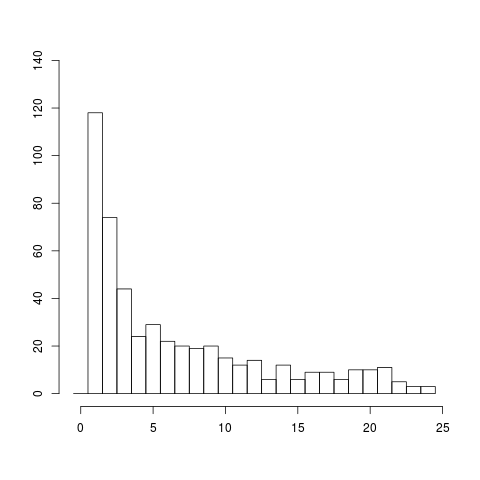
\includegraphics[width=0.6\textheight,  clip=]{../FIGURES/FigFisherHist-0} \\
        \onslide<2>
        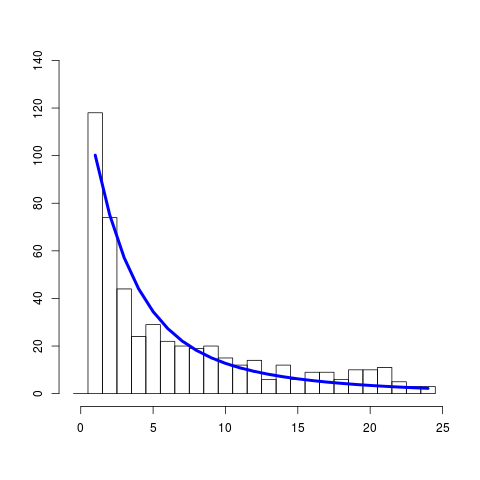
\includegraphics[width=0.6\textheight,  clip=]{../FIGURES/FigFisherHist-1} \\
        \onslide<3->
        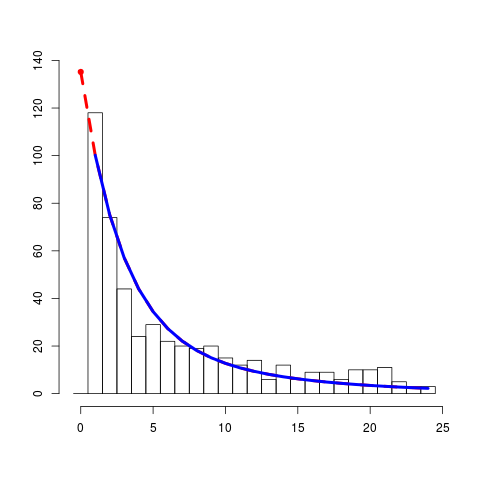
\includegraphics[width=0.6\textheight,  clip=]{../FIGURES/FigFisherHist-2} \\
      \end{overprint}
    \end{tabular}
  \end{tabular}
  
  \onslide+<5->{
    \bigskip
    \paragraph{'Non parametric'=} parametric mixture
    $
    g(\cdot) = \sum_k \pi_k f_k(\cdot).
    $
  }
}

%====================================================================
\frame{ \frametitle{Species abundance distribution (SAD)}
  
  \paragraph{Some classical distributions:}
  \begin{itemize}
  \item \emphase{Poisson}; 
  \item \emphase{Log-normal} (\refer{DoB08}); 
  \item \emphase{Poisson-Gamma} (\refer{FCW43},
    \refer{HDP10}) = Poisson counts with Gamma intensities;
  \item \emphase{Mixture} of discrete distributions $f(\cdot; \gamma)$:
    $$
    g(x) = \int f(x; \gamma) \pi(\gamma) \dd \gamma
    $$
  \end{itemize}


  \pause\bigskip
  \paragraph{Interest of the SAD:}
  \begin{itemize}
  \item Modeling the SAD allows to \emphase{guaranty identifiability}.
  \item SAD provides the \emphase{saturation curve} 
    $$
    \Pr\{X_i > 0\}
    $$
    which is useful to design experiments.
  \end{itemize}

}

%====================================================================
\frame{ \frametitle{In this talk}
  
  \paragraph{Goal:}
      \begin{itemize}
      \item Provide an \emphase{estimate of $g(0)$}
      \item With \emphase{confidence bounds}.
      \end{itemize}

  \pause \bigskip
  \tableofcontents

}


%====================================================================
\section{Bayesian averaging of mixture models}
\frame{ \frametitle{Bayesian averaging of mixture models}

  Joint work with 
  \begin{itemize}
  \item S. Li-Thiao-T�, 
  \item J.-J. Daudin 
  \end{itemize}
}
%====================================================================

%====================================================================
\subsection*{Mixture models}
\frame{ \frametitle{Mixture models} 
  \paragraph{'Non-parametric' = mixture model:} \refer{NoP98}
  $$
  \pi(\gamma) = \sum_k \pi_k \delta_{\gamma_k}(\gamma) \quad \Rightarrow \quad
  g(x) = \sum_k \pi_k f(x; \gamma_k).
  $$

  \bigskip\pause
  \paragraph{Truncated mixture vs Mixture of truncated.} The
  distribution of the observed counts can be expressed in \emphase{two
    equivalent ways}:
  \begin{eqnarray}
    g^+(x) & = & \sum_k \pi_k f(x; \gamma_k) \left/ \left[ 1 -
        \sum_k \pi_k f(0; \gamma_k) \right]
        \right. \label{Eq:TruncMixt} \\
    \text{or} \qquad g(x) & = & \sum_k \emphase{\pi^+_k f^+}(x;
        \gamma_k). \label{Eq:MixtTrunc} 
  \end{eqnarray}

  }

%====================================================================
\frame{ \frametitle{Incomplete data model}
  
  A mixture model can be rewritten as:
  \begin{eqnarray*}
    (Z_i)_i \text{ iid:} \quad Z_i & \sim & \Mcal(1; \pi), \\
    (X_i)_i \text{ indep. } | (Z_i)_i: \quad X_i|Z_i=k & \sim &
    f^+(\cdot; \gamma_k)
  \end{eqnarray*}
  where $Z_i$ is the \emphase{unknown group to which species $i$
    belongs}. 

  \bigskip
  \begin{tabular}{cc}
    \hspace{-.5cm}
    \begin{tabular}{p{.5\textwidth}}
      \paragraph{Notations:}
      \begin{eqnarray*}
        X = (X_i)_i &  & \text{\emphase{observed} counts}, \\
        Z = (Z_i)_i &  & \text{\emphase{unobserved} groups,} \\
        \theta = (\pi, \gamma) &  & \text{\emphase{parameter} }
%        : \pi = (\pi_k)_k, \; \gamma =
        (\gamma_k)_k.  
      \end{eqnarray*}
      
      \medskip\pause
      \begin{itemize}
      \item We need get an \emphase{estimate $\widehat{\theta}$}
      \item or to calculate the \emphase{posterior $P(\theta|X)$}.
      \end{itemize}
    \end{tabular}
    & 
    \hspace{-.5cm}
    \begin{tabular}{p{.5\textwidth}}
      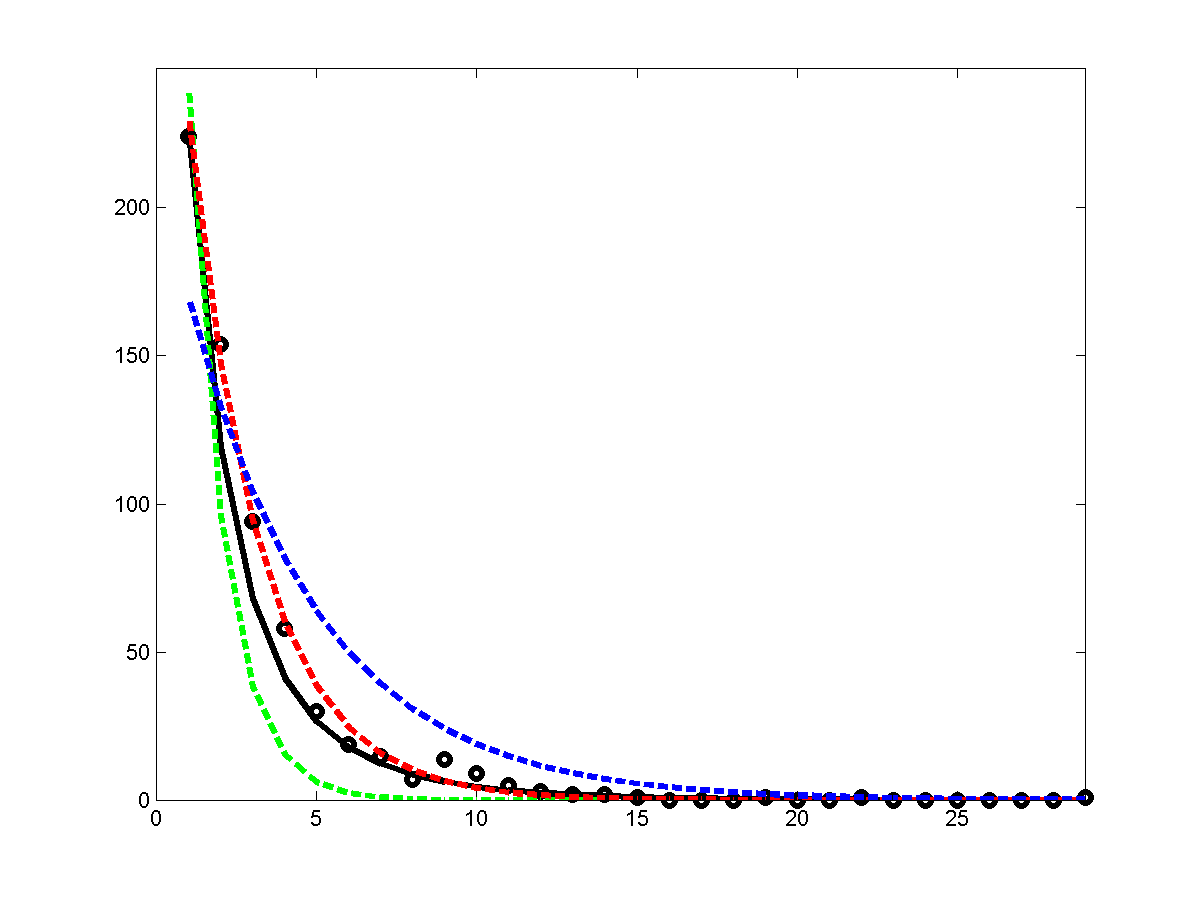
\includegraphics[width=.45\textwidth, 4=.height\textheight, clip=]{../FIGURES/SimMixtGeomComp}
    \end{tabular}
  \end{tabular}
  }

%==================================================================== 
\frame{ \frametitle{Inference}
%==================================================================== 
  \paragraph{Inference on truncated data:} 
  \begin{itemize}
  \item Inference of \emphase{mixture of truncated}
    \eqref{Eq:TruncMixt} is often easier than this of
    \emphase{truncated mixture} \eqref{Eq:MixtTrunc}.
  \item MLE estimates for \eqref{Eq:TruncMixt} and
    \eqref{Eq:MixtTrunc} are equivalent (\refer{BoK06}) in the Poisson
    case.
%   \item Truncated geometric $\Gcal$ are still geometric, whereas
%     truncated Poisson $\Pcal$ are not Poisson.
%   \item Precision of the estimates are not that easy to derive in the
%     frequentist context.
  \end{itemize}
  %\refer{BoK06,BeF08,DoB08,HDP10,SHB08}

  \bigskip\pause
  \paragraph{Bayesian inference}
  \begin{itemize}
  \item Bayesian inference provides \emphase{credibility interval}
    through the posterior $P(\theta|X)$.
  \item Exact Bayesian inference with incomplete data requires
    \emphase{computationally intensive MCMC}.
  \item \paragraph{Variational Bayes} provides an (optimal)
    approximation of the joint posterior $P(\theta, Z|X)$ .
%     as
%     $$
%     Q^*(\theta, Z) = \underset{Q \in \Qcal}{\arg\min} \;
%     KL\left[Q^*(\theta, Z), P(\theta, Z|X) \right]
%     $$
%     in the context of the exponential family with conjugate priors.
  \end{itemize}

  }

%====================================================================
\subsection*{Variational Bayes}
%====================================================================
\frame{ \frametitle{Exponential family / Conjugate prior}

  \paragraph{Exponential family:}
  $$
  P(X, Z|\theta) \propto \exp[\emphase{\psi(\theta)}' u(X,
  Z)]
  $$
  includes distributions like geometric, Poisson, truncated
  geometric ... but \emphase{not truncated Poisson} (while they can
  still be handled...)

  \bigskip\pause
  \paragraph{Conjugate prior.}
  $$
  P(\theta) \propto \exp[\emphase{\psi(\theta)}' \nubf] 
  $$
  that is 
  \begin{itemize}
  \item Dirichlet for the multinomial distribution ($Z$), 
  \item Gamma for Poisson or Beta for the geometric ($X|Z$),
  \end{itemize}
  $$
  \Rightarrow \qquad P(\theta|X, Z) \propto
  \exp\{\emphase{\psi(\theta)}' [u(X, Z) + \nubf] \}.
  $$

  }

%====================================================================
\frame{ \frametitle{Variational Bayes E-M}

  \paragraph{Best approximation.} As $P(\theta, Z|X)$ is
  intractable, we look for the best 'manageable' approximation:
  \begin{eqnarray*}
    Q^*(\theta, Z) & = & \underset{Q \in \Qcal}{\arg\min} \;
    \emphase{KL}[\emphase{Q(Z, \theta)}; \emphase{P(Z,
    \theta|X)}] \\ 
    & = & \underset{Q \in \Qcal}{\arg\min} \; \Hcal(\emphase{Q}) -
    \Esp_{\emphase{Q}} [\log \emphase{P(X, Z, \theta)}] + \text{cst}
  \end{eqnarray*}

  \bigskip\bigskip\pause
  \paragraph{Factorisable distributions.} When considering the class
  $$
  \Qcal = \{Q(\theta, Z) = \emphase{\Qt(\theta)
    \QZ(Z)}\}, 
  $$
  the optimal $Q^* \in \Qcal$ can be recovered via (\refer{BeG03})
  \begin{eqnarray*}
    \text{'M'-step:} \quad \Qt(\theta) 
    & \propto 
    & \exp \left(\psi(\theta)'
      \left[ \Esp_{\emphase{\QZ}}u(X, Z) + \nubf \right]
    \right) \\ 
    \\
    \text{'E'-step:} \quad \QZ(Z)     
    & \propto     
    & \exp ( \Esp_{\emphase{\Qt}}\psi(\theta)' u(X, Z) ]
  \end{eqnarray*}

  }

%====================================================================
\subsection*{Bayesian model averaging}
\frame{ \frametitle{Bayesian model averaging}
%==================================================================== 

  \paragraph{Number of components.} 
  \begin{itemize}
  \item The number of components \emphase{$K$ is unknown} 
  \item ... but the existence of a '\emphase{true}' number of
    component is \emphase{questionable}.
  \end{itemize}
  
  \bigskip\pause
  \paragraph{Bayesian model averaging (BMA).} Consider a parameter of interest $\Delta = \Delta(\theta)$ that can be defined for a series of models $1, \dots, K \dots$. Denoting
  $$
  \Esp(\Delta | X, K) = \int \Delta(\theta) P(\theta | X, K) \dd \theta
  $$
  we have
  $$
  \Esp(\Delta | X) = \sum w_k \Esp(\Delta | X, K)
  $$
  where 
  $$
  w_K = P(K | X),
  $$
  the calculation of which is an issue.
  }

%====================================================================
\frame{ \frametitle{Evaluating the weights}

%   \paragraph{Theoretical weights.} We should compute
%   $$
%   w_K = P(K|X) \propto P(X| K) = \frac{P(X|\theta, K)
%     P(\theta|K)}{\emphase{P(\theta|X, K)}}
%   $$
%   which has no close-form, but a \emphase{plug-in} estimate is
%   straightforward:
%   $$
%   \widehat{w}_K  \propto \frac{P(X|\theta,
%     K) P(\theta|K)}{\emphase{\Qt^*(\theta | K)}}
%   $$
% 
%   \bigskip\pause
  \paragraph{Optimal variational approximation.} Optimal weights can
  be obtained by direct minimisation of
  $$
  KL[Q(\emphase{K, Z, \theta}), P(\emphase{K, Z, \theta} | X)]
  $$
  to get (\refer{VMR12})
  \begin{eqnarray*}
  \tilde{w}_K 
%   & := & Q^*(K) \\
%   & \propto & \exp\left\{-KL[Q^*(Z, \theta|K); P(Z, \theta|X, K)] + \log P(X, K)\right\} \\
  & \propto & P(K |X) \exp\left\{-KL[Q^*(Z, \theta|K); P(Z, \theta|X, K)] \right\}.
  \end{eqnarray*}
  which combines
  \begin{itemize}
   \item the posterior probability of the model $P(K|X)$
   \item with the quality of the variational inference within the model
  \end{itemize}
  (although none of the two can be computed).


  }

%====================================================================
\subsection*{Microbial diversity in human gut}
\frame{ \frametitle{Microbial diversity in human gut (\refer{TML09})}
%==================================================================== 

  \paragraph{Fit of different geometric mixtures $K = 1, \dots 5$:}
  $\widehat{\theta}_K =$ mode of $\Qt(\theta)$.
  $$
  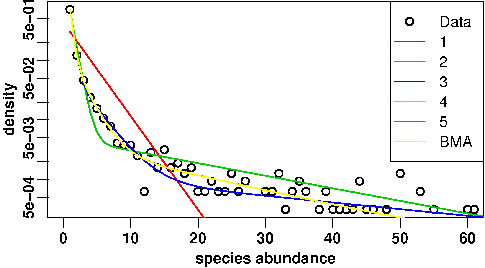
\includegraphics[width=0.75\textwidth, clip=]{../FIGURES/TapMondot2}
  $$
  $$
  \emphase{\text{Mixture: }} \widehat{g}^{+K}(x) = \sum_k
    \widehat{\pi}_K f^+(x; \widehat{\gamma}_K), 
  \qquad
  \emphase{\text{BMA: }} \widetilde{g}^+(x) = \sum_K w_K \widehat{f}^{+K}(x). 
  $$
  }

%==================================================================== 
\frame{ \frametitle{Saturation curve}

  \paragraph{Reverse use of $\widetilde{f}^+(x)$:} Design of NGS
  metagenomics experiment
  $$
  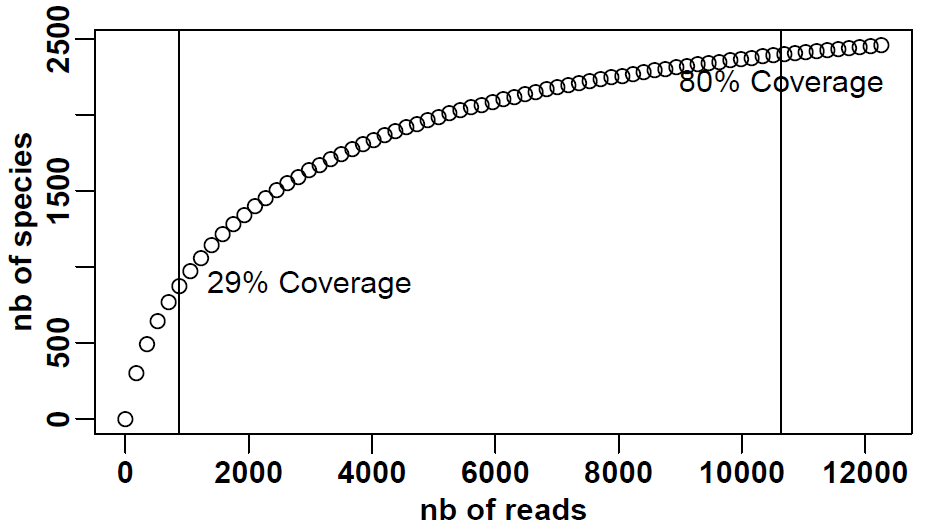
\includegraphics[width=0.75\textwidth, clip=]{../FIGURES/Rarefaction}
  $$
  \refer{LDR12}

  }

%====================================================================
\subsection*{Credibility interval for the number of species}
\frame{ \frametitle{Confidence interval for the number of species}
%==================================================================== 

  \paragraph{Geometric distribution.} The proportion of absent species
  under the geometric distribution is
  $$
  \widehat{g}(0) = \widehat{\gamma}
  $$
  for which the \emphase{approximate posterior $Q^*_K(\gamma)$ is a
    Beta distribution}.

  \bigskip\pause
  \paragraph{Mixture of geometric,} we get
  $$
  \widehat{g}_K(0) = \sum_{k=1}^K \widehat{\pi}_k \widehat{\gamma}_k.
  $$

  \bigskip\pause
  \paragraph{Number of absent species.} The Horwitz-Thomson is
  $$
  \widehat{C}_K = c / [1 - \widehat{g}_K(0)].
  $$

  \bigskip
  \paragraph{BMA} can also be applied:
  $$
  \widetilde{C} = \sum_{K=1}^{K_{\max}} w_K \widehat{C}_K.
  $$
  }

%====================================================================
\subsection*{Importance sampling}
\frame{ \frametitle{Importance sampling}
%==================================================================== 

  \paragraph{Approximate posterior.} 
  \begin{itemize}
  \item Variational Bayes only provides an \emphase{approximate
      posterior $\Qt(\theta)$}.
  \item which is known to often \emphase{under-estimate} the posterior
    variances.
  \end{itemize}

%   \bigskip\pause
%   \paragraph{Monte-Carlo estimate.} Taking \emphase{$(\theta^b)_b \text{
%       iid} \sim P(\theta)$}, we have
%   $$
%   \int_{\Ical} P(X|\theta) P(\theta) \dd \theta
%   \simeq 
%   \frac1B \sum_{\theta^b \in \Ical} P(X|\theta^b) 
%   =: 
%   \widehat{P}(\theta \in \Ical|X) 
%   $$
%   but the variance is large when $P(\theta)$ is \emphase{far from}
%   $P(\theta|X)$.
    
  \bigskip\bigskip\pause
  \paragraph{Importance sampling (IS).} For any distribution $Q$, taking $\{\theta^b\}$ iid $\sim Q$, 
  \begin{eqnarray*}
  \int_{\Ical} P(X|\theta) {P(\theta)} \dd \theta 
  & = & \int_{\Ical} P(X|\theta)
  \emphase{\frac{P(\theta)}{Q(\theta)}} Q(\theta) \dd \theta \\
  & \simeq & \frac1B \sum_{\theta^b \in \Ical} 
  \emphase{\frac{P(\theta^b)}{Q(\theta^b)}} P(X|\theta^b) 
  \quad =: \quad \widehat{P}(\theta \in \Ical|X).
%   \frac1{P(X)} \int P(X|\theta) \frac{P(X)}{Q(X)}
%   Q(\theta) \dd \theta \simeq \frac1B \sum_b P(X|\theta^b)
%   \frac{P(X)}{Q(X)} =: \widehat{P}(\theta|X).
  \end{eqnarray*}
  The variance gets smaller when $Q$ gets closer to $P(\theta|X)$. \\
  \smallskip
  \ra The variational approximation \emphase{$Q^*(\theta)$ can be used as a proxy.}
    
  }

%====================================================================
\frame{ \frametitle{Approximate posterior distribution}
  
  A Gibbs sampler is used as a \emphase{gold standard for $\widehat{P}(\cdot|X)$}. \\
  \bigskip
  \begin{tabular}{cc}
    \begin{tabular}{c}
      \paragraph{Simulated data:} $\widehat{g}(0)$ \vspace{.15cm} \\      
      \includegraphics[width=0.45\textwidth, height=0.325\textwidth]{../FIGURES/vbem3} \\
      \refer{LDR12} \pause 
    \end{tabular} 
    &
    \begin{tabular}{c}
    \paragraph{Human gut:} $\widehat{C}_0 = 25,700$ \\
      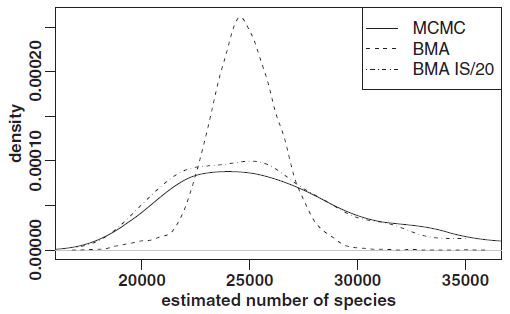
\includegraphics[height=.5\textheight, width=0.45\textwidth,  clip=]{../FIGURES/LDR12-Fig6} \\
      $\text{CI}_{95\%} = [19,421; 36,355]$. \\
    \end{tabular}
  \end{tabular}
  }

%====================================================================
\section{A 'true' non-parametric estimate}
\frame{\frametitle{A 'true' non-parametric estimate}

  Joint work with 
  \begin{itemize}
  \item C. Durot, 
  \item F. Koladjo, 
  \item S. Huet
  \end{itemize}
}
%====================================================================

%====================================================================
\subsection*{Convexity assumption}
\frame{\frametitle{Convexity assumption}
%====================================================================
  \begin{tabular}{ccc}
    \hspace{-3cm}
    \begin{tabular}{p{.25\textwidth}}
      ~\\
      Most real-life SAD
      seem to be convex. \\ 
      \onslide+<2>{
	\paragraph{\ra Assumption:} 
	$$
	g(\cdot) \text{ is convex}.
	$$
      }
    \end{tabular}
    &     \hspace{-3cm}
    \begin{tabular}{p{.5\textwidth}}
      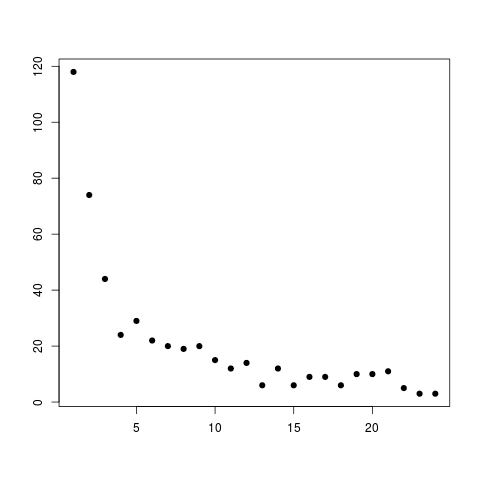
\includegraphics[width=.3\textwidth]{../FIGURES/butterfly}
    \end{tabular}
    &     \hspace{-3cm}
    \begin{tabular}{p{.5\textwidth}}
      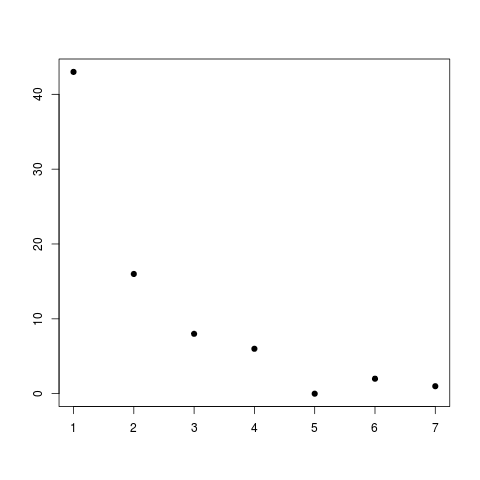
\includegraphics[width=.3\textwidth]{../FIGURES/cottontail}
    \end{tabular}
    \\
    \hspace{-.5cm}
    \begin{tabular}{p{.5\textwidth}}
      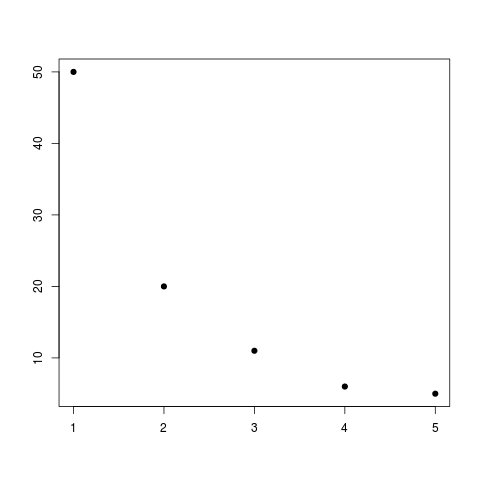
\includegraphics[width=.3\textwidth]{../FIGURES/insects}
    \end{tabular}
    &     \hspace{-3cm}
    \begin{tabular}{p{.5\textwidth}}
      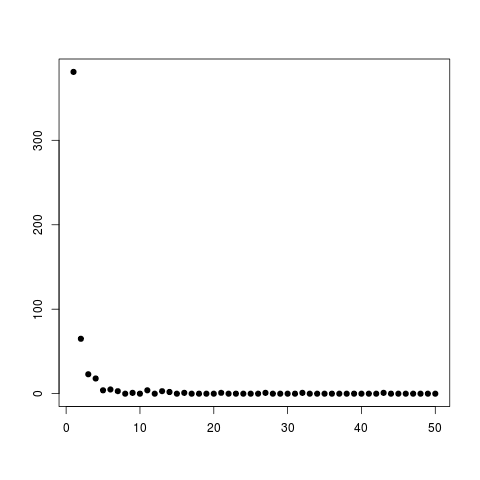
\includegraphics[width=.3\textwidth]{../FIGURES/microbial}
    \end{tabular}
    &     \hspace{-3cm}
    \begin{tabular}{p{.5\textwidth}}
      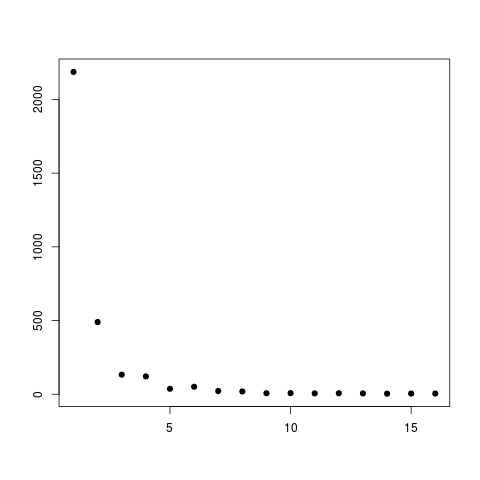
\includegraphics[width=.3\textwidth]{../FIGURES/EST}
    \end{tabular}
  \end{tabular}
  }


%====================================================================
\subsection*{Decomposition of convex distributions}
\frame{\frametitle{Decomposition of convex distributions}
%====================================================================
  
  \begin{tabular}{cc}
    \hspace{-.5cm}
    \begin{tabular}{p{.4\textwidth}}
      Any convex distribution $g$ can be decomposed as a mixture 
      $$
      g(x) = \sum_j \pi_j T_j(x)
      $$
      where the $T_j$ are triangular distributions\footnote{this also holds for continuous convex distributions.}
      $$
      T_j(x) = \frac{2 (j-x)}{j(j+1)}.
      $$
    \end{tabular}
    & 
    \hspace{-.5cm}
    \begin{tabular}{p{.5\textwidth}}
      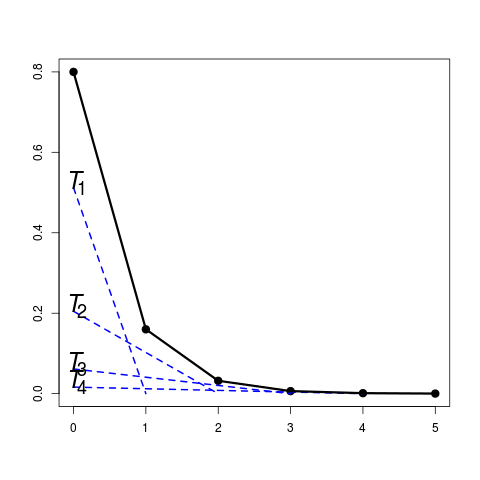
\includegraphics[width=.55\textwidth]{../FIGURES/GeomTri-p8}
    \end{tabular}
  \end{tabular}  
  }

%====================================================================
\subsection*{Convex SAD}
\frame{\frametitle{A definition of convex SAD}
  
  \paragraph{Mixture interpretation.} Species are spread into groups
  \begin{eqnarray*}
   (Z_i) \text{ iid} & \sim & \Mcal(1; \pi) \\
   (X_i) \text{ indep} | (Z_i): \quad X_i|Z_i=j & \sim & T_j
  \end{eqnarray*}

  \bigskip \pause
  \paragraph{Interpretation of group 1.} $T_1$ is Dirac mass on 0 \\
  \smallskip
  \ra Species from group 1 can only display $X_i = 0$ \\
  \smallskip
  \ra Such species can be thought of as ... absent species.

  \bigskip\bigskip \pause
  \paragraph{Definition.} (\refer{DKH12}) $g$ is a convex SAD if 
  \begin{enumerate}[($i$)]
   \item $g$ is convex discrete distribution.
   \item The proportion of $T_1$ is null: $\pi_1 = 0$.
  \end{enumerate}

  }

%===================================================================
\frame{\frametitle{Non-parametric (convex) estimate of $g$}
  
  \paragraph{Empirical truncated distribution.} 
  $$
  \widetilde{g}_n^+(x) = n^{-1} \sum_i \Ibb\{X_i = x\}, \qquad x > 0
  $$

  \bigskip
  \paragraph{Least-square truncated convex SAD estimate.}
  $$
  \widehat{g}_n^+ = \arg\min_{g \in \Ccal} \|g - \widetilde{g}_n^+ \|^2
  $$
  where $\Ccal$ denotes the set of truncated convex SAD.

  \bigskip\bigskip\pause
  \paragraph{Inference.}
  $\widehat{g}_n^+$ can be obtained via an extension of the support reduction algorithm (\refer{GJW01}) to an unknown support for $g^+$.
  }


%===================================================================
\frame{\frametitle{Some properties of $\widehat{g}^+_n$}

  \begin{enumerate}
   \item The support $\widehat{s}_n$ of $\widehat{g}^+$ is finite. \\~ \pause
   \item If $g^+$ is convex, $\widehat{g}^+$ is consistent at rate $\sqrt{n}$:
   $$
   \sqrt{n} \|\widehat{g}^+ - g^+\|_r  = O_P(1), \qquad \text{for } r \geq 2.
   $$\\~ \pause
   \item If $g^+$ is not convex, $\widehat{g}^+$ converge towards the projection of $g^+$ onto $\Ccal$:
   $$
   \sqrt{n} \|\widehat{g}^+ - \Pi_\Ccal g^+\|_r  = O_P(1), \qquad \text{for } r \geq 2.
   $$ \\~ \pause
   \item Absolute moments are larger for $\widehat{g}^+$ than for $\widetilde{g}^+$.
  \end{enumerate}
  }

%===================================================================
\frame{\frametitle{Sensitivity to non-convexity}

  \includegraphics[width=1\textwidth, height=.7\textheight]{../FIGURES/L2Poiloss} 

  Estimated $\ell_2$ loss for the empirical pdf \textcolor{red}{$\widehat{g}$} and the convex estimate $\widehat{g}$ as a function of $n$ for set of non-convex Poisson distribution ($\lambda \leq 2 - \sqrt2$).
  
%   \caption{Left: Three different Poisson distributions.
%     Solid ({\bf --}):$\lambda=\lambda^*$, dashed (-\,-):$\lambda=.8$,
%     dotted ($\cdots$):$\lambda=1$. Right: empirical $\ell_2$-loss as a function
%     of $n$. Black: $\widetilde{p}_n$, \textcolor{red}{red}:
%     $\widehat{p}_n$. \label{Fig:Pois}}

  }

%===================================================================
\subsection*{Proportion of unobserved species}
\frame{\frametitle{Proportion of unobserved species}

  \paragraph{Estimate of $g(0)$.} Using the definition of convex SAD (i.e. $\pi_1 = 0$):
  $$
  \widehat{g}(0) = \frac{\widehat{\theta}}{1+\widehat{\theta}} \qquad \text{where} \quad \widehat{\theta} = 2\widehat{g}^+(1) - \widehat{g}^+(2).
  $$ 

  \bigskip \pause
  \paragraph{Ongoing work.}
  \begin{itemize}
   \item Asymptotic variance of $\widehat{\theta}$: no closed form. \\~
   \item $\sqrt{n}(\widehat{\theta} - \theta)$ converges in distribution towards a non-standard distribution\footnote{The asymptotic distribution of $\widetilde{\theta}$ is standard}. \\
   \ra Bootstrap procedure.
  \end{itemize}
  }

% %===================================================================
% \frame{\frametitle{Some simulations}
% 
%   \begin{tabular}{cc}
%     \begin{tabular}{p{.2\textwidth}}
%       \paragraph{MSE for $g(0)$.} \\
%       \\
%       Empirical \\
%       dist. $\widetilde{g}$ \\
%       \\
%       vs \\
%       \\
%       \textcolor{red}{Convex} \\
%       estimate $\widehat{g}$
%       
%     \end{tabular}
%     & 
%     \hspace{-1cm}
%     \begin{tabular}{c}
%       \includegraphics[width=.8\textwidth, height=.8\textheight]{../FIGURES/P0MSEr}
%     \end{tabular}
%   \end{tabular}
%   }

%===================================================================
\frame{\frametitle{Some examples}

  \begin{tabular}{ccc}
    \begin{tabular}{p{.15\textwidth}}
      \textcolor{blue}{Poisson mixture} \\
      ~\\ ~\\ 
      and
    \end{tabular}
    & 
    \begin{tabular}{c}
      \includegraphics[width = .3\textwidth]{../FIGURES/FCW43-Butterfly-p0} 
    \end{tabular}
    &
    \begin{tabular}{c}
      \includegraphics[width = .3\textwidth]{../FIGURES/NoP98-p0} 
    \end{tabular}
    \\
    \begin{tabular}{p{.15\textwidth}}
      \textcolor{red}{convex} \\ 
      \textcolor{red}{estimate}
    \end{tabular}
    & 
    \begin{tabular}{c}
      \includegraphics[width = .3\textwidth]{../FIGURES/BoS05-Accident-p0}
    \end{tabular}
    &
    \begin{tabular}{c}
      \includegraphics[width = .3\textwidth]{../FIGURES/Wan10-p0} 
    \end{tabular}
  \end{tabular}
  }

%====================================================================
\frame{  \frametitle{Sensitivity to truncation}

As SAD are often long-tailed, \refer{ChS04} suggest truncation at some $\tau$ to infer $g(0)$.

\begin{center}
  \begin{tabular}{cccccc}
    $\tau$&$\widehat C_{mCNP}$&$\widehat C_{u}$ & $\widehat C_{UNP}$&$\widehat C_{WL}$&$\widehat C_{CONV}$\\
    \hline  
    $10$ & $716$ &$715$ &$715$ &$716$ &$782$\\                           
    $11$ & $711$ &$715$ &$715$ &$739$ &$782$\\                            
    $12$ & $729$ &$723$ &$722$ &$730$ &$782$\\                       
    $13$ & $731$ &$724$ &$724$ &$728$ &$782$\\                        
    $14$ & $726$ &$723$ &$723$ &$724$ &$782$\\                           
    $15$ & $724$ &$722$ &$722$ &$724$ &$782$\\                            
    $20$ & $721$ &$718$ &$718$ &$725$ &$782$\\                         
    $24$ & $721$ &$719$ &$719$ &$722$ &$782$\\
  \end{tabular}
\end{center}

Estimates of $N$ on Fisher's butterfly data. \\

$\widehat N_{mCNP}$, $\widehat N_{u}$,  $\widehat N_{UNP}$ and $\widehat N_{WL}$ reported from \refer{WaL05}.

}

%====================================================================
\section*{Conclusion}
\frame{ \frametitle{Conclusion \& Future works}
%==================================================================== 

  \paragraph{Species abundance} is an old statistical problem revisited by metagenomics.

  \bigskip\pause
  \paragraph{First estimate:} Parametric with Bayesian inference 
  \begin{itemize}
  \item Mixture models \ra flexible modeling of the SAD;
  \item Variational Bayes Model Averaging \ra approximate posterior distribution;
  \item Importance sampling \ra exact posterior, less computationally demanding than MCMC.
  \end{itemize}

  \bigskip\pause
  \paragraph{Second estimate:} Non-parametric with frequentist inference
  \begin{itemize}
  \item Convexity \ra natural assumption for SAD;
  \item Triangular decomposition \ra definition of convex SAD;
  \item Asymptotic distribution of $\widehat{g}(0)$ \ra under study.
  \end{itemize}

  }


%====================================================================
{\tiny
  \bibliography{/media/donnees/Biblio/AST,/media/donnees/Biblio/ARC,/media/donnees/Biblio/SSB}
  \bibliographystyle{/media/donnees/LATEX/astats}
  %\bibliographystyle{plain}
  }

%====================================================================
%====================================================================
\end{document}
%====================================================================
%====================================================================

  \begin{tabular}{cc}
    \hspace{-.5cm}
    \begin{tabular}{p{.5\textwidth}}
    \end{tabular}
    & 
    \hspace{-.5cm}
    \begin{tabular}{p{.5\textwidth}}
    \end{tabular}
  \end{tabular}

